\documentclass{article}
\usepackage{amsfonts} % For \mathbb
\usepackage{amsmath} % For align*
\usepackage{enumitem} % For customisable list labels
\usepackage{graphicx} % For images
\usepackage{siunitx} % For units
\graphicspath{{./images/}}

\renewcommand{\Im}{\operatorname{Im}}
\renewcommand{\Re}{\operatorname{Re}}

\title{Advanced Engineering Mathematics Systems of Differential Equations by Dennis G. Zill Notes}
\author{Chris Doble}
\date{August 2023}

\begin{document}

\maketitle

\tableofcontents

\setcounter{section}{9}
\section{Systems of Linear Differential Equations}

\subsection{Theory of Linear Systems}

\begin{itemize}
  \item A system of the form \begin{align*}
          \frac{d x_1}{d t} & = g_1(t, x_1, x_2, \ldots, x_n) \\
          \frac{d x_2}{d t} & = g_2(t, x_1, x_2, \ldots, x_n) \\
          \vdots                                              \\
          \frac{d x_n}{d t} & = g_n(t, x_1, x_2, \ldots, x_n)
        \end{align*} is called a \textbf{first-order system}.

  \item When each of the functions $g_n(t, x_1, x_2, \ldots, x_n)$ is linear in the dependent variables $x_1, x_2, \ldots, x_n$, we get the \textbf{normal form} of a first-order system of linear equations \begin{align*}
          \frac{d x_1}{d t} & = a_{11}(t) x_1 + a_{12}(t) x_2 + \ldots + a_{1n}(t) x_n + f_1(t)  \\
          \frac{d x_2}{d t} & = a_{21}(t) x_1 + a_{22}(t) x_2 + \ldots + a_{2n}(t) x_n + f_2(t)  \\
          \vdots                                                                                 \\
          \frac{d x_n}{d t} & = a_{n1}(t) x_1 + a_{n2}(t) x_2 + \ldots + a_{nn}(t) x_n + f_n(t). \\
        \end{align*} Such a system is called a \textbf{linear system}.

  \item When $f_i(t) = 0$ for $i = 1, 2, \ldots, n$ the linear system is said to be \textbf{homogeneous}, otherwise it's \textbf{nonhomogenous}.

  \item If $\mathbf{X}$, $\mathbf{A}(t)$, and $\mathbf{F}(t)$ denote the matrices \begin{align*}
          \mathbf{X}    & = \begin{pmatrix}
                              x_1(t) \\
                              x_2(t) \\
                              \vdots \\
                              x_n(t)
                            \end{pmatrix}                             \\
          \mathbf{A}(t) & = \begin{pmatrix}
                              a_{11}(t) & a_{12}(t) & \ldots & a_{1n}(t) \\
                              a_{21}(t) & a_{22}(t) & \ldots & a_{2n}(t) \\
                              \vdots    &           &        & \vdots    \\
                              a_{n1}(t) & a_{n2}(t) & \ldots & a_{nn}(t)
                            \end{pmatrix} \\
          \mathbf{F}(t) & = \begin{pmatrix}
                              f_1(t) \\
                              f_2(t) \\
                              \vdots \\
                              f_n(t)
                            \end{pmatrix}
        \end{align*} then homogeneous linear systems can be written \[\mathbf{X}' = \mathbf{A} \mathbf{X}\] and nonhomogeneous linear systems can be written \[\mathbf{X}' = \mathbf{A} \mathbf{X} + \mathbf{F}.\]

  \item A \textbf{solution vector} on an interval $I$ is any column matrix \[\mathbf{X} = \begin{pmatrix}
            x_1(t) \\
            x_2(t) \\
            \vdots \\
            x_n(t)
          \end{pmatrix}\] whose entries are differentiable functions satisfying the linear system on the interval.

  \item The entries of a solution vector can be considered a set of parametric equations that define a curve in $n$-space. Such a curve is called a \textbf{trajectory}.

  \item The problem of solving \[\mathbf{X}' = \mathbf{A}(t) \mathbf{X} + \mathbf{F}(t)\] subject to \[\mathbf{X}(t_0) = \mathbf{X}_0\] is an \textbf{initial value problem} in matrix form.

  \item The \textbf{superposition principle} states that if $\mathbf{X}_1, \mathbf{X}_2, \ldots, \mathbf{X}_n$ are solution vectors of a homogeneous linear system on an interval $I$, then \[\mathbf{X} = c_1 \mathbf{X}_1 + c_2 \mathbf{X}_2 + \ldots + c_n \mathbf{X}_n\] where $c_n$ are arbitrary constants is also a solution.

  \item If $\mathbf{X}_1, \mathbf{X}_2, \ldots, \mathbf{X}_n$ are a set of solution vectors of a homogeneous linear system on an interval $I$, the set is said to be \textbf{linearly dependent} if there exist constants $c_1, c_2, \ldots, c_n$ not all zero such that \[c_1 \mathbf{X}_1 + c_2 \mathbf{X}_2 + \ldots + x_n \mathbf{X}_n = \mathbf{0}\] for every $t$ in the interval. Otherwise the set is said to be \textbf{linearly independent}.

  \item A set of solution vectors \[\mathbf{X}_1 = \begin{pmatrix}
            x_{11} \\
            x_{21} \\
            \vdots \\
            x_{n1}
          \end{pmatrix}, \quad \mathbf{X}_2 = \begin{pmatrix}
            x_{12} \\
            x_{22} \\
            \vdots \\
            x_{n2}
          \end{pmatrix}, \quad \ldots, \quad \mathbf{X}_n = \begin{pmatrix}
            x_{1n} \\
            x_{2n} \\
            \vdots \\
            x_{nn}
          \end{pmatrix}\] is linearly independent on an interval $I$ if the \textbf{Wronskian} \[W(\mathbf{X}_1, \mathbf{X}_2, \ldots, \mathbf{X}_n) = \begin{vmatrix}
            x_{11} & x_{12} & \ldots & x_{1n} \\
            x_{21} & x_{22} & \ldots & x_{2n} \\
            \vdots &        &        & \vdots \\
            x_{n1} & x_{n2} & \ldots & x_{nn}
          \end{vmatrix} \ne 0\] for every $t$ in the interval.

  \item Any set of $n$ linearly independent solution vectors of a homogeneous linear system on an interval $I$ is said to be a \textbf{fundamental set of solutions} on that interval.

  \item If $\mathbf{X}_1, \mathbf{X}_2, \ldots, \mathbf{X}_n$ are a fundamental set of solutions of a homogeneous linear system on an interval $I$, then the \textbf{general solution} of the system on that interval is \[\mathbf{X} = c_1 \mathbf{X}_1 + c_2 \mathbf{X}_2 + \ldots + c_n \mathbf{X}_n\] where $c_i$ are arbitrary constants.

  \item For nonhomogenous systems, a \textbf{particular solution} $\mathbf{X}_p$ on an interval $I$ is any vector, free from arbitrary parameters, whose entries are functions that satify the system.

  \item For nonhomogeneous systems, the \textbf{general solution} of the system on the interval is \[\mathbf{X} = \mathbf{X}_c + \mathbf{X}_p\] where $\mathbf{X}_c$ is the general solution of the associated homogeneous system (the \textbf{complementary function}) and $\mathbf{X}_p$ is a particular solution of the nonhomogeneous system.
\end{itemize}

\subsection{Homogeneous Linear Systems}

\subsubsection{Distinct Real Eigenvalues}

\begin{itemize}
  \item If $\mathbf{X}' = \mathbf{A} \mathbf{X}$ is a homogeneous linear system, $\lambda_1, \lambda_2, \ldots, \lambda_n$ are $n$ real, distinct eigenvalues of $\mathbf{A}$, and $\mathbf{K}_1, \mathbf{K}_2, \ldots, \mathbf{K}_n$ are the corresponding eigenvectors of $\mathbf{A}$, then \[\mathbf{X} = c_1 \mathbf{K}_1 e^{\lambda_1 t} + c_2 \mathbf{K}_2 e^{\lambda_2 t} + \ldots + c_n \mathbf{K}_n e^{\lambda_n t}\] is the general solution of the system.

  \item If a system of linear equations consists of variables $x$ and $y$, then the $x-y$ plane is called the \textbf{phase plane}.

  \item Solution vectors of a linear system can be considered parametric equations and plotted on the phase plane. These are called trajectories.

  \item When multiple trajectories are plotted in the phase plane, it's called a \textbf{phase portrait}.
\end{itemize}

\subsubsection{Repeated Eigenvalues}

\begin{itemize}
  \item If the coefficient matrix $\mathbf{A}$ of a linear system has an eigenvalue $\lambda$ of multiplicity $m$, it may be possible to find $m$ linearly independent eigenvectors $\mathbf{K}_1, \mathbf{K}_2, \ldots, \mathbf{K}_m$ associated with the eigenvalue in which case the $m$ solution vectors associated with the eigenvalue are \begin{align*}
          \mathbf{X}_1 & = \mathbf{K}_1 e^{\lambda t}  \\
          \mathbf{X}_2 & = \mathbf{K}_2 e^{\lambda t}  \\
          \vdots                                       \\
          \mathbf{X}_m & = \mathbf{K}_m e^{\lambda t}.
        \end{align*}

  \item If the coefficient matrix $\mathbf{A}$ of a linear system has an eigenvalue $\lambda$ of multiplicity $m$ and it's not possible to find $m$ linearly independent eigenvectors associated with the eigenvalue, then the $m$ solution vectors associated with the eigenvalue are \begin{align*}
          \mathbf{X}_1 & = \mathbf{K}_1 e^{\lambda t}                                                                                                                          \\
          \mathbf{X}_2 & = \mathbf{K}_1 t e^{\lambda t} + \mathbf{K_2} e^{\lambda t}                                                                                           \\
          \vdots                                                                                                                                                               \\
          \mathbf{X}_m & = \mathbf{K}_1 \frac{t^{m - 1}}{(m - 1)!} e^{\lambda t} + \mathbf{K}_2 \frac{t^{m - 2}}{(m - 2)!} e^{\lambda t} + \ldots + \mathbf{K}_m e^{\lambda t}
        \end{align*} where $\mathbf{K}_i$ are the solutions to the equations \begin{align*}
          (\mathbf{A} - \lambda \mathbf{I}) \mathbf{K}_1 & = \mathbf{0}          \\
          (\mathbf{A} - \lambda \mathbf{I}) \mathbf{K}_2 & = \mathbf{K}_1        \\
          \vdots                                                                 \\
          (\mathbf{A} - \lambda \mathbf{I}) \mathbf{K}_m & = \mathbf{K}_{m - 1}. \\
        \end{align*}
\end{itemize}

\subsubsection{Complex Eigenvalues}

\begin{itemize}
  \item If $\mathbf{A}$ is the coefficient matrix of a homogeneous linear system and it has a complex eigenvalue $\lambda = \alpha + i \beta$ and associated eigenvector $\mathbf{K}_1$, then \[\mathbf{X}_1 = \mathbf{K}_1 e^{\lambda t} \text{ and } \mathbf{X}_2 = \overline{\mathbf{K}}_1 e^{\overline{\lambda} t}\] are solutions of the system.

  \item The solutions above can be made real by writing them as \begin{align*}
          \mathbf{X}_1 & = [\mathbf{B}_1 \cos \beta t - \mathbf{B}_2 \sin \beta t] e^{\alpha t} \\
          \mathbf{X}_2 & = [\mathbf{B}_2 \cos \beta t + \mathbf{B}_1 \sin \beta t] e^{\alpha t}
        \end{align*} where $\mathbf{B}_1 = \Re (\mathbf{K}_1)$ and $\mathbf{B}_2 = \Im(\mathbf{K}_1)$.
\end{itemize}

\subsection{Solution by Diagonalization}

\begin{itemize}
  \item A homogeneous linear system $\mathbf{X}' = \mathbf{A} \mathbf{X}$ in which each $x_i'$ is expressed as a linear combination of $x_1, x_2, \ldots, x_n$ is said to be \textbf{coupled}. If each $x_i'$ is expressed solely in terms of $x_i$ the system is said to be \textbf{uncoupled}.

  \item Given a linear system $\mathbf{X' = A X}$, if the coefficient matrix $\mathbf{A}$ is diagonalisable such that $\mathbf{P^{-1} A P = D}$ then the system can be solved by:

        \begin{enumerate}
          \item Substituting $\mathbf{X = P Y}$ which gives $\mathbf{P Y' = A P Y}$ or \\ $\mathbf{Y' = P^{-1} A P Y = D Y}$

          \item Because $\mathbf{D}$ is a diagonal matrix with $\mathbf{A}$'s eigenvalues along the diagonal, this means the solutions to $\mathbf{Y' = D Y}$ are \[\mathbf{Y} = \begin{pmatrix}
                    c_1 e^{\lambda_1 t} \\
                    c_2 e^{\lambda_2 t} \\
                    \vdots              \\
                    c_n e^{\lambda_n t}
                  \end{pmatrix}\]

          \item These solutions can then be substituted into $\mathbf{X = P Y}$ to solve for $\mathbf{X}$
        \end{enumerate}
\end{itemize}

\subsection{Nonhomogeneous Linear Systems}

\subsubsection{Undetermined Coefficients}

\begin{itemize}
  \item The \textbf{method of undetermined coefficients} can be applied to a linear system $\mathbf{X' = A X + F(t)}$ when the entries of $\mathbf{A}$ are constants and the entries of $\mathbf{F}(t)$ are constants, polynomials, exponential functions, sines and cosines, or finite sums and products of these functions.

  \item To apply the method of undetermined coefficients:

        \begin{enumerate}
          \item Solve the associated homogeneous linear system to find the complementary function $\mathbf{X}_c$.

          \item Assume the particular solution $\mathbf{X}_p$ has the same form as $\mathbf{F}(t)$.

          \item Substitute the trial solution into the system and solve for the unknowns.

          \item The general solution is $\mathbf{X} = \mathbf{X_c + X_p}$.
        \end{enumerate}

  \item If $\mathbf{F}(t)$ contains a term that's present in the complementary function, that term needs to be adjusted (similar to how you multiply by $x^n$ in the method of undetermined coefficients for ODEs). The textbook doesn't cover the rules for this.
\end{itemize}

\subsubsection{Variation of Parameters}

\begin{itemize}
  \item If $\mathbf{X}_1, \mathbf{X}_2, \ldots, \mathbf{X}_n$ is a fundamental set of solutions of the homogeneous linear system $\mathbf{X' = A X}$ on an interval $I$, then the general solution is \[\mathbf{X} = c_1 \mathbf{X}_1 + c_2 \mathbf{X}_2 + \ldots + c_n \mathbf{X}_n\] which can also be written \[\mathbf{X} = \mathbf{\Phi}(t) \mathbf{C} = \begin{pmatrix}
            \mathbf{X}_1 & \mathbf{X}_2 & \ldots & \mathbf{X}_n
          \end{pmatrix} \mathbf{C}\] where $\mathbf{\Phi}(t)$ is called a \textbf{fundamental matrix} and $\mathbf{C}$ is a column vector containing the arbitrary constants $c_1, c_2, \ldots, c_n$.

  \item A fundamental matrix:

        \begin{itemize}
          \item always has an inverse, and

          \item has the property that $\mathbf{\Phi}'(t) = \mathbf{A} \mathbf{\Phi}(t).$
        \end{itemize}

  \item The \textbf{method of variation of parameters} finds a particular solution to a nonhomogeneous linear system by replacing column vector of unknown constants $\mathbf{C}$ with a column vector of functions \[\mathbf{U}(t) = \begin{pmatrix}
            u_1(t) \\
            u_2(t) \\
            \vdots \\
            u_n(t)
          \end{pmatrix}\] such that $\mathbf{X}_p = \mathbf{\Phi}(t) \mathbf{U}(t)$ is a particular solution to the system.

  \item $\mathbf{U}(t)$ can be calculated as \[\mathbf{U}(t) = \int \mathbf{\Phi}^{-1}(t) \mathbf{F}(t) \,dt\] so \[\mathbf{X}_p = \mathbf{\Phi}(t) \int \mathbf{\Phi}^{-1}(t) \mathbf{F}(t) \,dt\] and \[\mathbf{X} = \mathbf{X}_c + \mathbf{X}_p = \mathbf{\Phi}(t) \mathbf{C} + \mathbf{\Phi}(t) \int \mathbf{\Phi}^{-1}(t) \mathbf{F}(t) \,dt.\]

  \item When solving initial value problems via the method of variation of parameters where you're given $\mathbf{X}(t_0) = \mathbf{X}_0$, the column vector of arbitrary constants $\mathbf{C}$ can be calculated as \[\mathbf{C} = \mathbf{\Phi}^{-1}(t_0) \mathbf{X}_0.\]
\end{itemize}

\subsubsection{Diagonalization}

\begin{itemize}
  \item If the coefficient matrix $\mathbf{A}$ in a nonhomogeneous linear system \\ $\mathbf{X' = A X + F}(t)$ is diagonalizable, the system can be solved by:

        \begin{enumerate}
          \item Substituting $\mathbf{X = P Y}$ which gives $\mathbf{P Y' = A P Y + F}(t)$ or \\ $\mathbf{Y' = P^{-1} A P Y + P^{-1} F}(t)$ or $\mathbf{Y' = D Y + G}$

          \item Because $\mathbf{D}$ is a diagonal matrix with $\mathbf{A}$'s eigenvalues along the diagonal and $\mathbf{G = P^{-1} F}(t)$ this means $\mathbf{Y' = D Y + G(t)}$ is a set of $n$ uncoupled equations of the form \[\begin{pmatrix}
                    y_1'   \\
                    y_2'   \\
                    \vdots \\
                    v_n'
                  \end{pmatrix} = \begin{pmatrix}
                    \lambda_1 y_1 + g_1(t) \\
                    \lambda_2 y_2 + g_2(t) \\
                    \vdots                 \\
                    \lambda_n y_n + g_n(t)
                  \end{pmatrix}\]

          \item These equations can be solved and substituted into $\mathbf{X = P Y}$ to solve for $\mathbf{X}$.
        \end{enumerate}
\end{itemize}

\subsection{Matrix Exponential}

\begin{itemize}
  \item The linear first-order differential equation $x' = a x$ has a general solution $x = c e^{a t}$. Similarly, the system $\mathbf{X' = A X}$ has a general solution $\mathbf{X} = e^{\mathbf{A} t} \mathbf{C}$ where $e^{\mathbf{A} t}$ is an $n \times n$ matrix given by the \textbf{matrix exponential} and $\mathbf{C}$ is a $n \times 1$ matrix of arbitrary constants.

  \item The matrix exponential is defined as \[e^{\mathbf{A} t} = \sum_{k = 0}^\infty \mathbf{A}^k \frac{t^k}{k!}.\]

  \item The exponential of a diagonal matrix \[\mathbf{A} = \begin{pmatrix}
            a_{11} & 0      & \ldots & 0      \\
            0      & a_{22} & \ldots & 0      \\
            \vdots &        &        & \vdots \\
            0      & 0      & \ldots & a_{nn}
          \end{pmatrix}\] is \[e^{\mathbf{A} t} = \begin{pmatrix}
            e^{a_{11} t} & 0            & \ldots & 0            \\
            0            & e^{a_{22} t} & \ldots & 0            \\
            \vdots       &              &        & \vdots       \\
            0            & 0            & \ldots & e^{a_{nn} t}
          \end{pmatrix}.\]

  \item The nonhomogeneous system $\mathbf{X' = A X + F}$ has a general solution \[\mathbf{X} = \mathbf{X_c} + \mathbf{X}_p = e^{\mathbf{A} t} \mathbf{C} + e^{\mathbf{A} t} \int e^{-\mathbf{A} t} \mathbf{F} \,dt\] where \[e^{-\mathbf{A} t} = (e^{\mathbf{A} t})^{-1}\] is the inverse of $e^{\mathbf{A} t}$.

  \item A matrix exponential can be calculated with the inverse Laplace transform \[e^{\mathbf{A} t} = \mathcal{L}^{-1} \{ (s \mathbf{I} - \mathbf{A})^{-1} \}.\]

  \item A matrix exponential or that of one of its eigenvalues can be calculated as \[e^{\mathbf{A} t} = \sum_{j = 0}^{n - 1} \mathbf{A}^j b_j(t) \text{ or } e^{\lambda t} = \sum_{j = 0}^{n - 1} \lambda^j b_j(t)\] where $b_j(t)$ are the same for both expressions. This means that for an $n x n$ matrix with $n$ distinct eigenvalues the expressions for $e^{\lambda_1 t}, e^{\lambda_2 t}, \ldots, e^{\lambda_n t}$ give $n$ equations with $n$ unknowns ($b_j(t)$). Solving for the $b_j(t)$ and substituting them into the expression for $e^{\mathbf{A} t}$ allows us to calculate the matrix exponential.
\end{itemize}

\section{Systems of Nonlinear Differential Equations}

\subsection{Autonomous Systems}

\begin{itemize}
  \item A system of first-order differential equations is called \textbf{autonomous} when the system can be written in the form \begin{align*}
          \frac{d x_1}{d t} & = g_1(x_1, x_2, \ldots, x_n)  \\
          \frac{d x_2}{d t} & = g_2(x_1, x_2, \ldots, x_n)  \\
          \vdots                                            \\
          \frac{d x_n}{d t} & = g_n(x_1, x_2, \ldots, x_n),
        \end{align*} i.e. the independent variable $t$ doesn't appear on the right-hand side of each equation.

  \item Any autonomous second-order differential equation $x'' = g(x, x')$ can be written as the autonomous system \begin{align*}
          x' & = y        \\
          y' & = g(x, y).
        \end{align*}

  \item A system with $n = 2$ is called a \textbf{plane autonomous system} and its equations \begin{align*}
          \frac{d x}{d t} & = P(x, y) \\
          \frac{d y}{d t} & = Q(x, y)
        \end{align*} define a vector field in a region of the plane that represents a particle's velocity at a given point $(x, y)$.

  \item If $P(x, y)$, $Q(x, y)$, and the first-order partial derivatives $\partial P / \partial x$, $\partial P / \partial y$, $\partial Q / \partial x$, and $\partial Q / \partial y$ are continuous in the region $R$ of the plane, then a solution to the plane autonomous system may be one of three types:

        \begin{enumerate}
          \item A \textbf{constant solution} $x(t) = x_0, y(t) = y_0$ (or $\mathbf{X} = \mathbf{X}_0$ for all $t$). Also known as a \textbf{critical/stationary point} or an \textbf{equilibrium solution}.

          \item A solution $x = x(t), y = y(t)$ defines an \textbf{arc} — a plane curve that does not cross itself. Crossing itself would imply that the system has two solutions at a single point.

          \item A periodic solution $x = x(t), y = y(t)$. A periodic solution is called a \textbf{cycle}. If $p$ is the period of the solution, then $\mathbf{X}(t + p) = \mathbf{X}(t)$.
        \end{enumerate}

  \item Sometimes it's not possible to find explicit expressions for the solutions of nonlinear systems in one coordinate system, but it is in another. If we take the expressions for polar coordinates \begin{align*}
          r^2    & = x^2 + y^2           \\
          \theta & = \arctan \frac{y}{x}
        \end{align*} and differentiate them with respect to $t$ \begin{align*}
          \frac{d r}{d t}      & = \frac{1}{r} \left( x \frac{d x}{d t} + y \frac{d y}{d t} \right)    \\
          \frac{d \theta}{d t} & = \frac{1}{r^2} \left( -y \frac{d x}{d t} + x \frac{d y}{d t} \right)
        \end{align*} sometimes substituting a system's expressions for $\frac{d x}{d t}$ and $\frac{d y}{d t}$ into these equations allow them to be solved.
\end{itemize}

\subsection{Stability of Linear Systems}

\begin{itemize}
  \item Considering a plane system as the velocity field of a particle, if a particle is placed at $\mathbf{X}_0$ near a critical point $\mathbf{X}_1$ and the particle eventually moves to $\mathbf{X}_1$ or remains near it (e.g. circles), then $\mathbf{X}_1$ is said to be \textbf{locally stable}. If it's not possible to find a neighborhood in which the particle remains near $\mathbf{X}_1$ then it is said to be \textbf{unstable}.

  \item If $\mathbf{A}$ is an $n \times n$ matrix, the \textbf{trace} of $\mathbf{A}$ is the sum of the main diagonal entries.

  \item If $\mathbf{A}$ is the $2 \times 2$ coefficient matrix of a homogeneous linear system then its characteristic equation can be written as \[\det (\mathbf{A} - \lambda \mathbf{I}) = \lambda^2 - \tau \lambda - \Delta = 0\] where $\tau$ is its trace and $\Delta$ is its determinant. Using the quadractic equation we find that \[\lambda = \frac{\tau \pm \sqrt{\tau^2 - 4 \Delta}}{2}\] and thus the nature of $\mathbf{A}$'s eigenvalues are determined by the expression \[\tau^2 - 4 \Delta.\]

  \item The phase portrait of a system of two linear differential equations is determined by the eigenvalues and eigenvectors. There are three cases:

        \begin{enumerate}
          \item The eigenvalues are real and distinct ($\tau^2 - 4 \Delta > 0$) so the general solution has the form $\mathbf{X} = c_1 \mathbf{K}_1 e^{\lambda_1 t} + c_2 \mathbf{K}_2 e^{\lambda_2 t}$.

                \begin{itemize}
                  \item If both eigenvalues are negative $\lim_{t \rightarrow \infty} \mathbf{X} = \mathbf{0}$ and $\mathbf{X}$ will approach $\mathbf{0}$ from one of two directions determined by $\mathbf{K}_1$ and $\mathbf{K}_2$. In this case a critical point is called a \textbf{stable node}.

                  \item If both eigenvalues are positive $\mathbf{X}$ becomes unbounded as $t$ increases, moving in one of two directions determined by $\mathbf{K}_1$ and $\mathbf{K}_2$. In this case a critical point is called a \textbf{unstable node}.

                  \item If the eigenvalues have opposite signs $\mathbf{X}$ approaches $\mathbf{0}$ from the direction of the eigenvector associated with the negative eigenvalue, then becomes unbounded in the direction of the other eigenvector. In this case a critical point is called a \textbf{saddle point}.
                \end{itemize}

          \item There is a single real and repeated eigenvalue ($\tau^2 - 4 \Delta = 0$). If $\lambda < 0$ then $\mathbf{X}$ approaches $\mathbf{0}$ from a direction determined by the eigenvector(s) and the critical point is called a \textbf{degenerate stable node}. If $\lambda > 0$ then $\mathbf{X}$ moves away from $\mathbf{0}$ in the same direction and the critical point is called a \textbf{degenerate unstable node}.

          \item The eigenvalues are complex ($\tau^2 - 4 \Delta < 0$).

                \begin{itemize}
                  \item If the eigenvalues are pure imaginary $\mathbf{X}$ moves in an ellipse with centre at the origin. The ellipses are all traversed in the same direction. In this case a critical point is called a \textbf{centre}.

                  \item When there is a nonzero real part the $e^{\alpha t}$ changes the radius over time. If $\alpha < 0$ the ellipse spirals towards $\mathbf{0}$ and is called a \textbf{stable spiral point}. If $\alpha > 0$ the ellipse spirals away from $\mathbf{0}$ and is called an \textbf{unstable spiral point}.
                \end{itemize}
        \end{enumerate}
\end{itemize}

\subsection{Linearization and Local Stability}

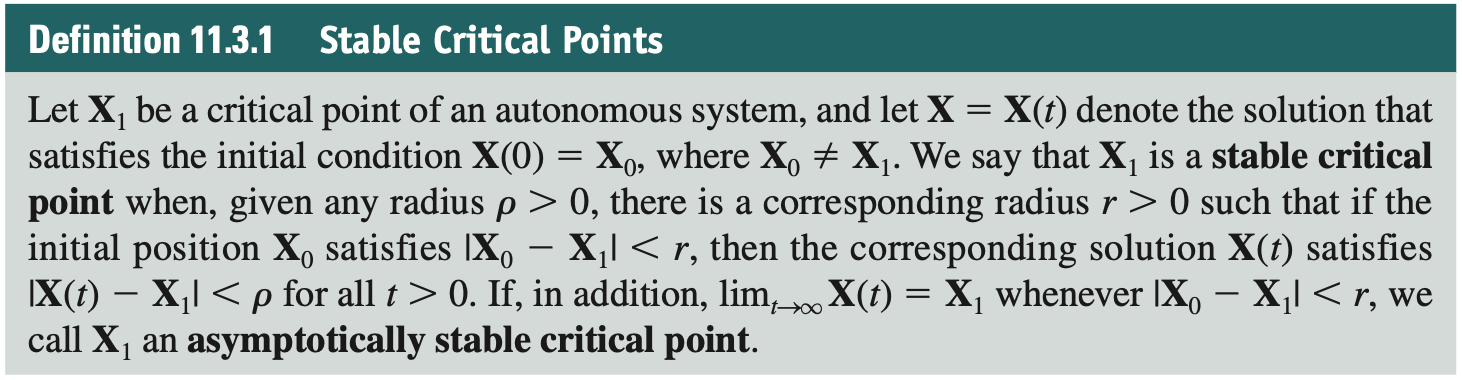
\includegraphics[scale=0.47]{stable-critical-points}

\begin{itemize}
  \item A critical point is called a \textbf{stable critical point} if for an arbitrary radius $\rho > 0$ it's always possible to find a radius $r > 0$ such that the solution is never more than $\rho$ units away from the critical point at all times.

  \item An \textbf{asymptotically stable critical point} is a critical point where the solution approaches the critical point as $t \rightarrow \infty$.
\end{itemize}

\noindent
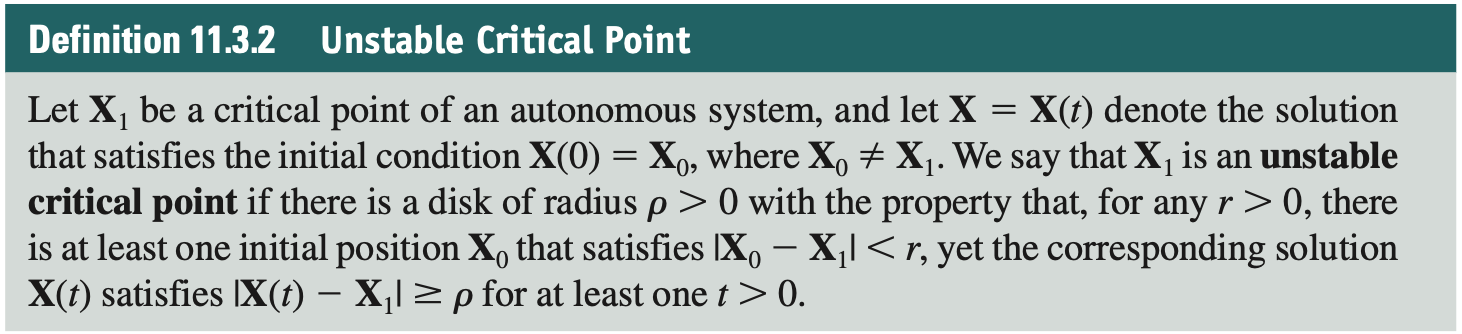
\includegraphics[scale=0.47]{unstable-critical-points}

\begin{itemize}
  \item An \textbf{unstable critical point} is a critical point that is not stable. In other words, for an arbitrary radius $\rho > 0$ it's always possible to find a solution whose initial position is less than $\rho$ units away from the critical point but eventually moves more than $\rho$ units away.
\end{itemize}

\noindent
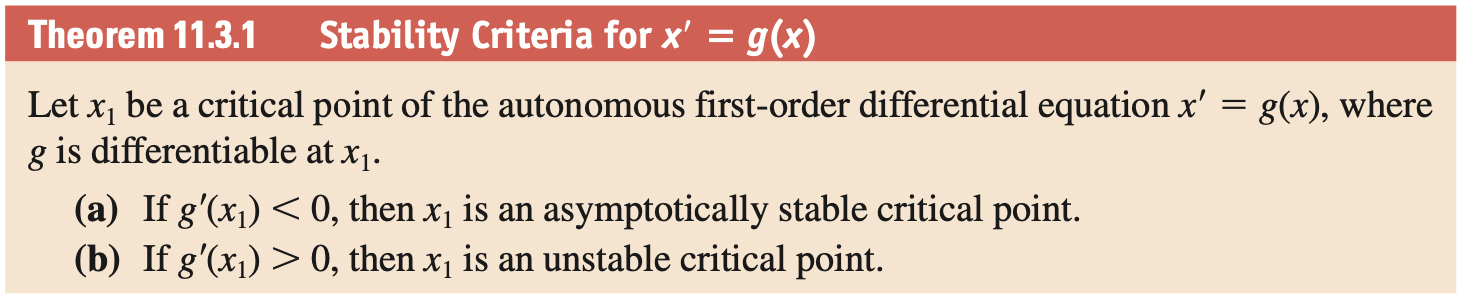
\includegraphics[scale=0.47]{stability-criteria-for-odes}

\begin{itemize}
  \item One way of thinking about theorem 11.3.1 is this:

        \begin{itemize}
          \item Consider the differential equation as representing the $x$-velocity of a particle. Because it's an autonomous equation, the particle's $x$-velocity is determined entirely by its $x$-coordinate. If $g(x) > 0$ the particle moves to the right. If $g(x) < 0$ it moves to the left.

          \item If $x_1$ is a critical point of the equation, then $g(x_1) = 0$.

          \item If $g'(x_1) < 0$ then $g(x) > 0$ just to the left of $x = x_1$ and $g(x) < 0$ just to the right.

          \item This means if the particle is displaced a small amount to the left of $x = x_1$ it will experience a restoring force to the right and vice versa if it's displaced to the right. This means $x = x_1$ is a stable critical point.

          \item Similarly, if $g'(x_1) > 0$ then $g(x) < 0$ just to the left of $x = x_1$ and $g(x) > 0$ just to the right. This is an unstable critical point.
        \end{itemize}

  \item An equation of the tangent plane to the surface $z = g(x, y)$ at $\mathbf{X}_1 = (x_1, y_1)$ is \[z = g(x_1, y_1) + \left. \frac{\partial g}{\partial x} \right|_{(x_1, y_1)} (x - x_1) + \left. \frac{\partial g}{\partial y} \right|_{(x_1, y_1)} (y - y_1).\]

  \item When $\mathbf{X}_1$ is a critical point of a plane autonomous system \begin{align*}
          x' & = P(x, y) \\
          y' & = Q(x, y)
        \end{align*} the system can be approximated in the neighborhood of the critical point with the tangent plane approximation, given by the linear system $\mathbf{X}' = \mathbf{A} (\mathbf{X} - \mathbf{X}_1)$ where \[\mathbf{A} = \begin{pmatrix}
            \left. \frac{\partial P}{\partial x} \right|_{(x_1, y_1)} & \left. \frac{\partial P}{\partial y} \right|_{(x_1, y_1)} \\
            \left. \frac{\partial Q}{\partial x} \right|_{(x_1, y_1)} & \left. \frac{\partial Q}{\partial y} \right|_{(x_1, y_1)}
          \end{pmatrix}\] is called the \textbf{Jacobian matrix}, denoted $\mathbf{g}'(\mathbf{X}_1)$.

  \item If we let $\mathbf{H} = \mathbf{X} - \mathbf{X}_1$ then $\mathbf{X}' = \mathbf{A} (\mathbf{X} - \mathbf{X}_1)$ becomes $\mathbf{H}' = \mathbf{A} \mathbf{H}$ and the critical points of the system can be analysed via the eigenvalues and eigenvectors of $\mathbf{A}$ as normal.
\end{itemize}

\noindent
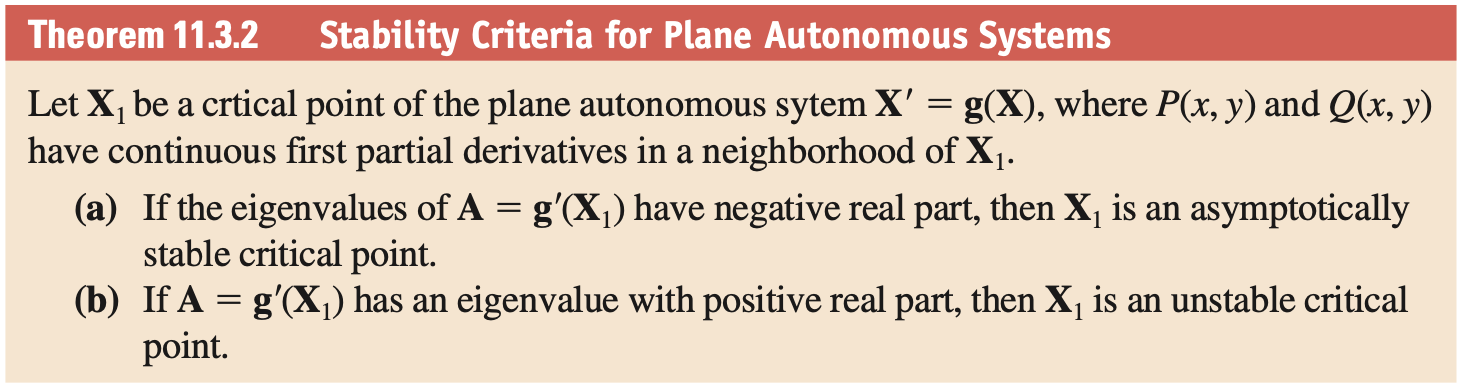
\includegraphics[scale=0.47]{stability-criteria-for-plane-systems}

\begin{itemize}
  \item Unlike with linear systems, it's not always possible to determine the geometric nature (stable node, stable spiral, etc.) of a critical point of a nonlinear autonomous system.

        \begin{itemize}
          \item If $\tau^2 = 4 \Delta$ (i.e. there is a single real and repeated eigenvalue) and $\tau > 0$ the critical point is unstable but we can't determine if it's an degenerate unstable node, unstable node, or unstable spiral. Similarly, if $\tau < 0$ the critical point is stable but we can't determine if it's a degenerate stable node, a stable node, or a stable spiral.

          \item If $\tau = 0$ and $\Delta > 0$ then the eigenvalues of the coefficient matrix are pure imaginary and the critical point may be a centre, a stable spiral, or an unstable spiral. It's not possible to classify it further.
        \end{itemize}

  \item The \textbf{phase-plane method} attempts to find $y$ as a function of $x$ by taking advantage of the fact that \[\frac{d y}{d x} = \frac{d y / d t}{d x / d t}.\] If you divide the expression for $d y / d t$ by that of $d x / d t$ it may be possible to solve the resulting ODE. The solution can then be graphed and the nature of critical points determined.
\end{itemize}

\subsection{Autonomous Systems as Mathematical Models}

\begin{itemize}
  \item
\end{itemize}

\end{document}